\documentclass[../report.tex]{subfiles}

\subsection{Specification}
	The application should be sectioned in to individual services following a microservices style architecture.  This allows for development of a single component independently from others and allows the mocking of APIs that are not yet implemented.  This also allows for faster iteration and integration testing.  In a production-like environment, this means that development and bug-fixing of components can be done locally unlike with a monolithic application.
	
	The application should also allow for deferred, batched or long-running tasks to be performed without interfering with the user experience.
	
	Data should be persistent and not susceptible to race conditions and access times should be minimised.
	
	It is a requirement that as much of the code is done in Python as possible.  This is to allow potential later utilisation of the code by others in the Department.
	
\subsection{Architecture Overview}
	Given the microservices style of application development chosen, it made sense to bundle each of the services in Docker containers.  Containers are similar to Virtual Machines (VMs) in that they allow for isolation of filesystems, memory and network between processes or groups of processes but by sharing an Operating System Kernel it removes the need to run a hypervisor.
	
	This also means development could utilise a tool called Docker Compose which allows for the running of a group of containers with their own virtual network on a workstation.  It also allows for the running of community containers such as PostgreSQL, Minio and Redis which are dependencies of the application without having to install and administer them.
	
	The user entry point to the application is served by the \textit{interface} service.  This provides a web based interface to the various backend components and rendering of graphs as well as acting as a reverse proxy to the various APIs behind the application.
	
	The \textit{observations} service is exposed via a mostly JSON based HTTP API.  It's primary responsibility is the storing accessing of raw observation files and events, as well as downsampling for rendering in a web browser.
	
	The \textit{SAX} service is exposed via a JSON based HTTP API.  Its purpose is to perform PAA and SAX operations on a given event and return data for rendering visualisations as well as the produced string from the SAX calculation.
	
	The \textit{Suffix} service is also behind a JSON based HTTP API.  It exists to store and query data with Suffix Trees.
	
	The \textit{worker} service exists to perform long running or compute heavy tasks asynchronously from the interface.  It is exposed via a message queue running on Redis (an in-memory key-value database) where the interface or other services can queue tasks.
	
	The HTTP/JSON APIs were written using Flask-Restplus, a Python framework based on Flask that allows for request and response definition using Python Decorators around classes and methods.  The framework allows for dynamic generation of a swagger.json a commonly used format for defining APIs.  Swagger also provides a user friendly HTML based interface for testing methods and calls during development and also doubles as API documentation.  An example of Swagger used on the Suffix Tree API is shown in \cref{fig:swagger}.
	
\begin{figure}[h]
	\centering
	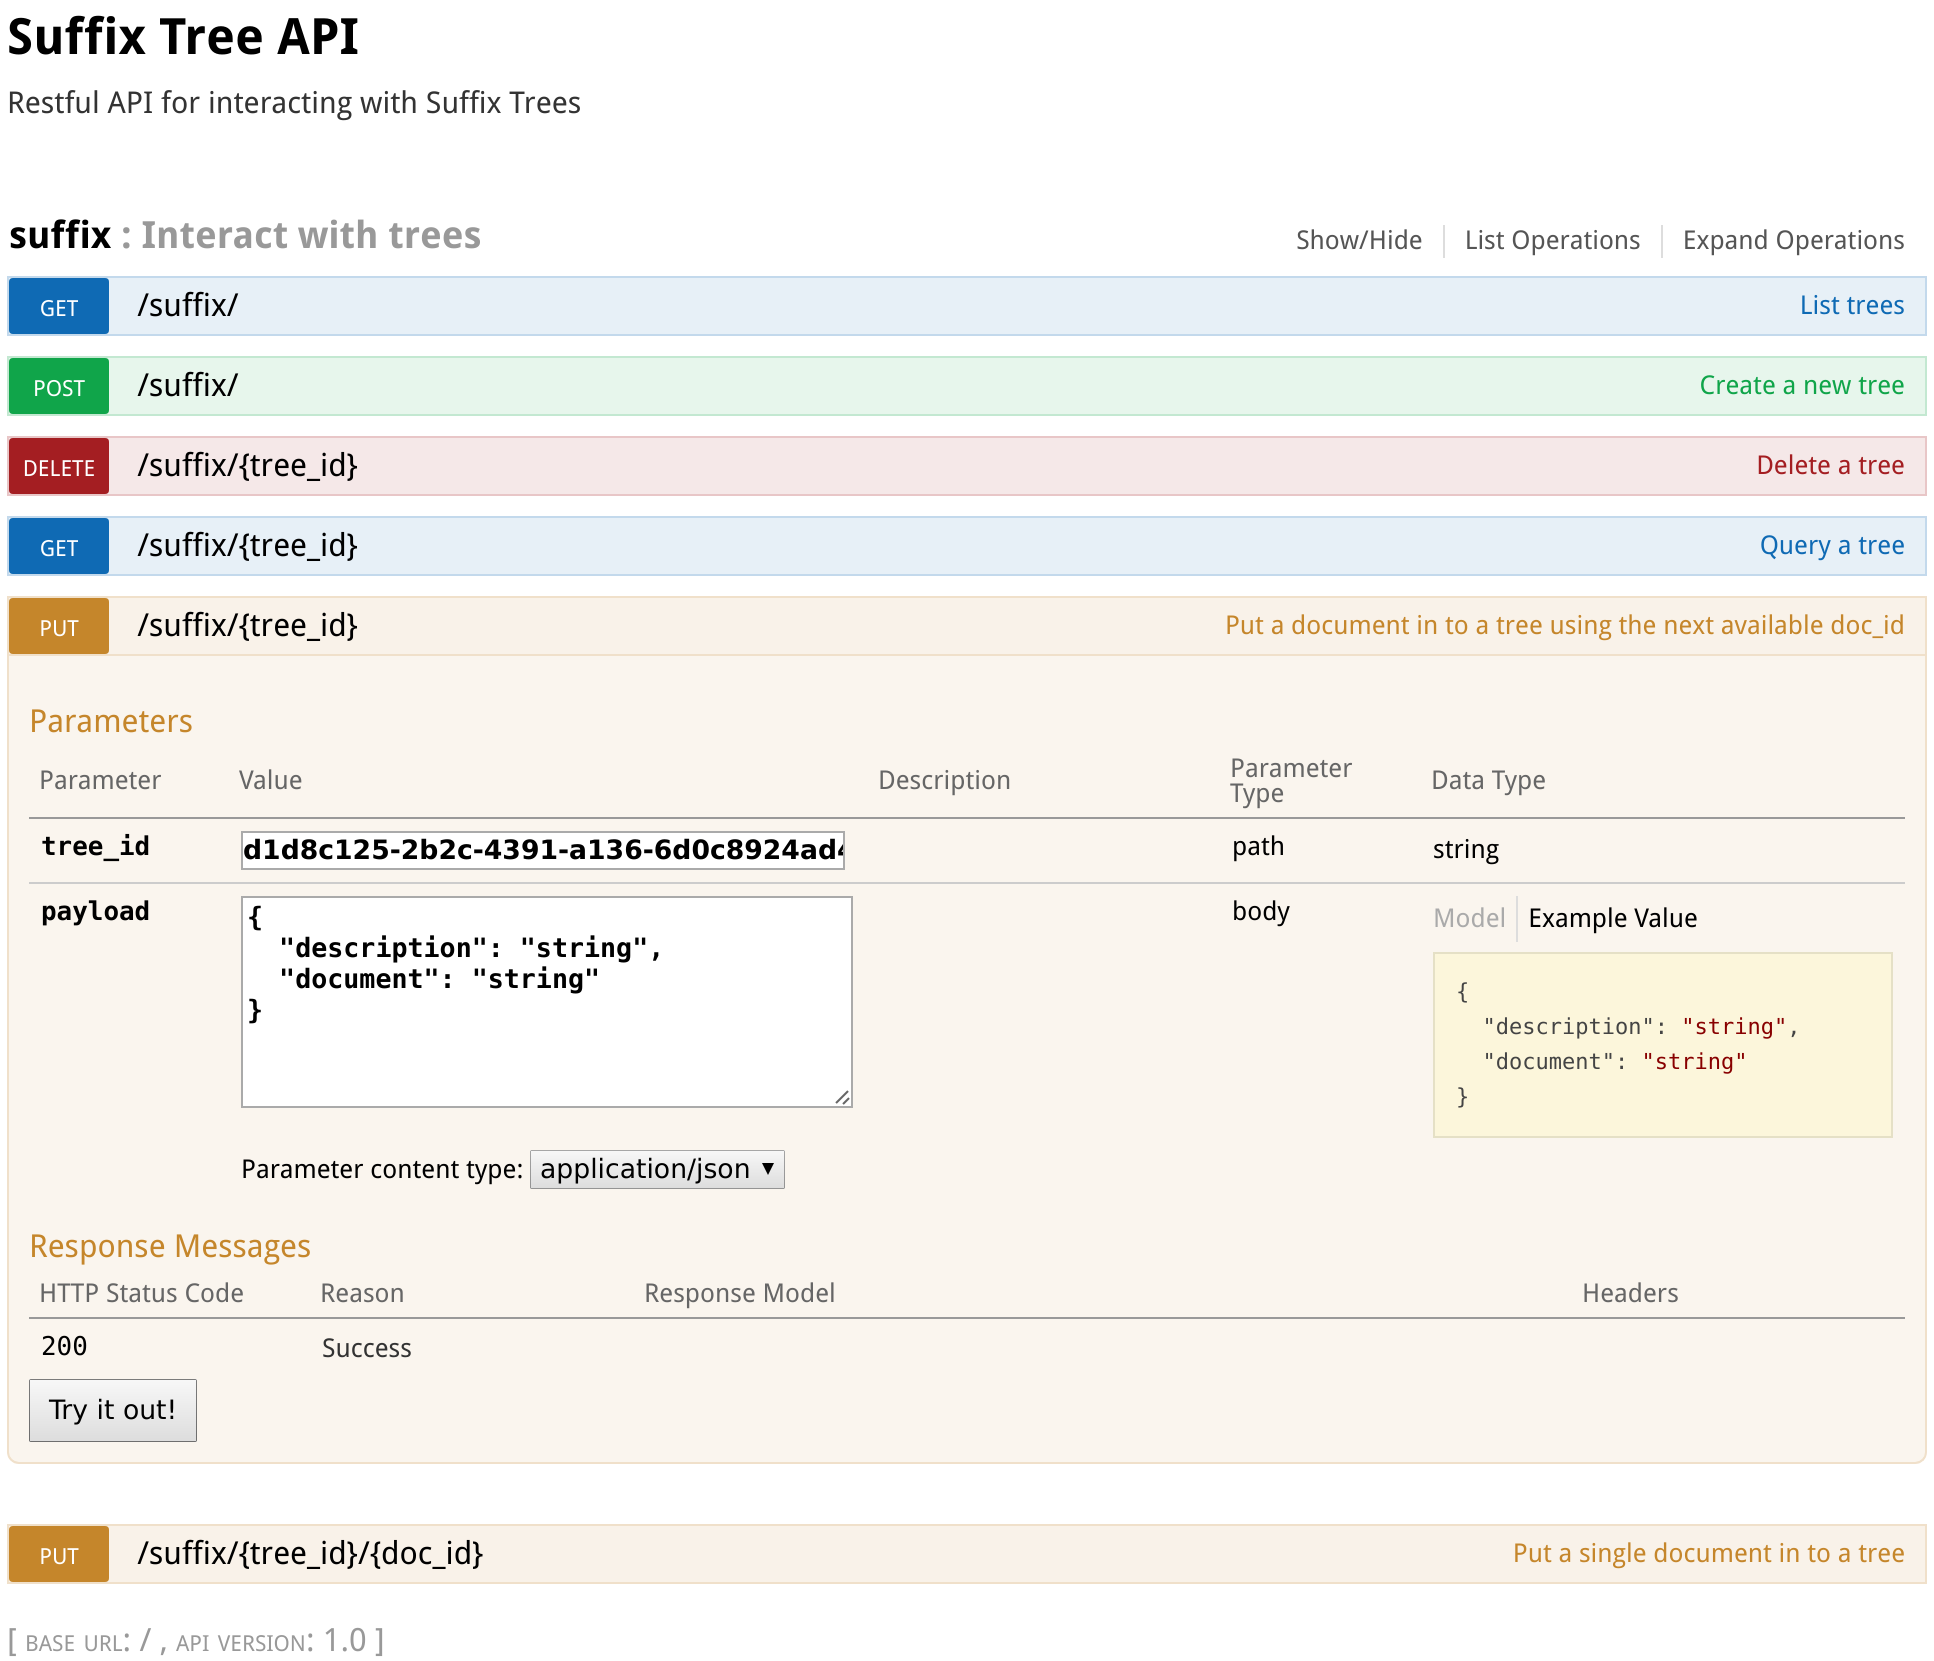
\includegraphics[width=1\linewidth]{img/swagger}
	\caption{Swagger interface for Suffix Tree API}
	\label{fig:swagger}
\end{figure}

	
	
\subsubsection{Interface}
	As mentioned previously, the interface to the application is web-based.  This serves two purposes; firstly it provides a unified experience across operating systems and secondly some of the processing can be memory and CPU intensive so is better suited for running on server hardware.
	
	The interface is served using Flask for Python.  Flask allows for dynamic request handling by converting URL paths directly in to function calls in Python.  It also supports HTML templating via Jinja2.  An module was written to act as a reverse proxy to expose various sections of the backend APIs to the browser.
	
	The view and control components of the interface were written in HTML (using Twitters Bootstrap) and Javascript (using AngularJS, Charts.js and c3.js).  AngularJS allows for two way data binding between the Broswers DOM and elements such as form inputs and renders with minimal additional code.  It also provides a mechanism for sending requests to the APIs exposed by the aforementioned Proxy module.  Chart.js and c3.js are two open source Javascript charting libraries that utilise features included in HTML5 used in this case for rendering observation data.

\subsubsection{Data Persistence}
	For the persistence of Metadata about observations, detected events and Suffix Trees, PostgreSQL was selected.  PostgreSQL is a performant and mature open-source Relational Database Management System (RDBMS).  Being a fully featured RDBMS means it brings ACID guarantees for data resilience and transaction management.
	
	For the persistence of Binary objects (such as Raw Observation Files and Suffix Trees), Minio was selected.  Minio is an open-source object storage application written in Golang designed to emulate the abilities of Amazons Simple Storage Service (S3).  It allows for arbitrary binary objects to be stored and retrieved remotely from \textit{buckets} of grouped resources.  In each bucket, an object has a unique name that can also emulate a filesystem path (e.g. \textit{bucket}/somedir/somefile).
	
	A wrapper class was written around Minio that provides Get, Put and Delete operations.  This interface was intentionally left simple so that it could be replaced easily by another object or file store.
	
\subsubsection{Observations API}

\subsubsection{SAX API}
\subsubsection{Suffix API}
\subsubsection{Deferred \& Batch Jobs}
	For the running of deferred and batch jobs, Celery (another Python based project) was selected.  It uses a message queue for receiving and dispatching jobs.  Celery allows for the definition of jobs as functions which can then be imported by other processes (in this case, mostly the user interface).  The application uses Redis as the message queue. It also allows for the chaining together of tasks to ensure order (e.g. event detection before SAX analysis) and the passing of results on to the next function in a functional programming style.
